\subsection{Objekt-Dateien einlesen}
Unter $"$Datei->Öffnen$"$ kann eine Objekt-Datei geöffnet werden. (siehe ~\ref{fig:DateiOeffnen})
\begin{figure}[ht!]
\centering
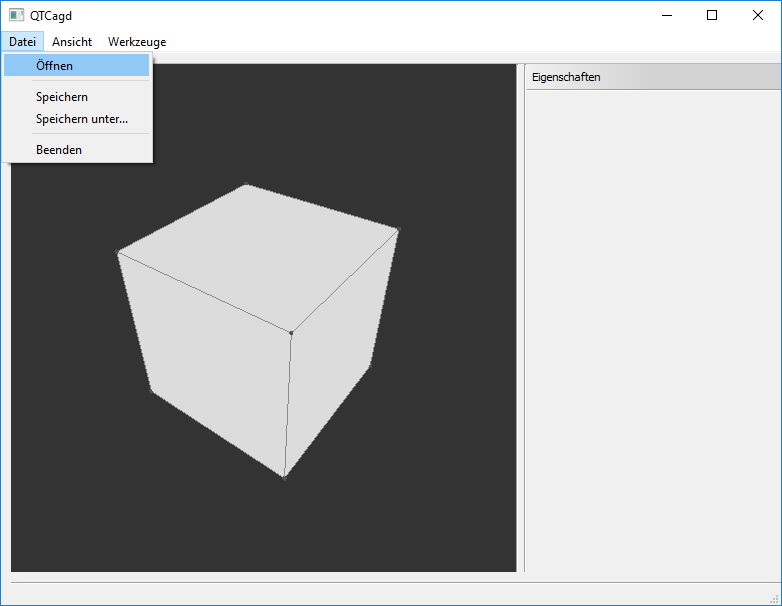
\includegraphics[width=0.6\linewidth]{content/pictures/0-DateiOeffnen}
\label{fig:DateiOeffnen}
\caption{}
\end{figure}
\subsection{Objekt-Dateien speichern}
Unter $"$Datei->Speichern$"$ oder mit $"$Datei->Speichern unter...$"$ kann eine Objekt-Datei gespeichert werden. (siehe ~\ref{fig:DateiSpeichern})

\begin{figure}[ht!]
	\centering
	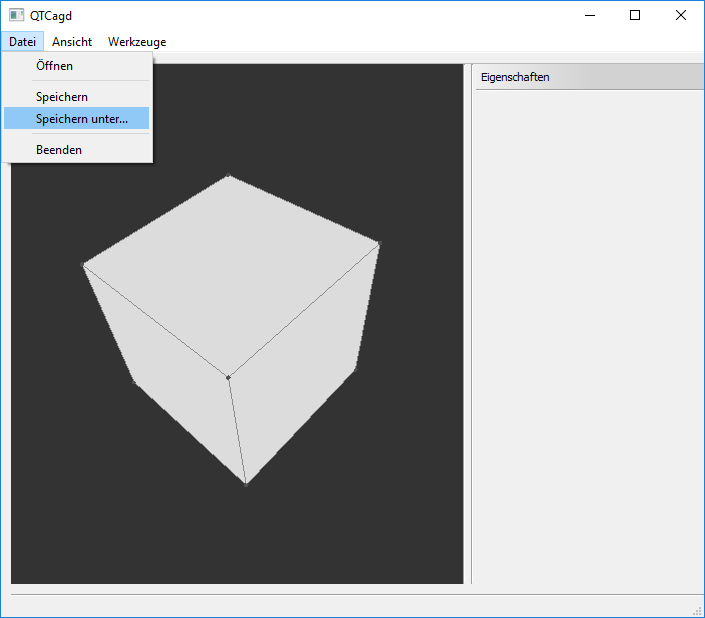
\includegraphics[width=0.6\linewidth]{content/pictures/1-DateiSpeichern}
	\label{fig:DateiSpeichern}
	\caption{}
\end{figure}

\subsection{Ansichtsmodi}
Es können 3 Ansichtsmodi aktiviert werden und zwar den $"$Vertex Mode$"$ oder den $"$Edge Mode$"$ oder den $"$Face Mode$"$. (siehe ~\ref{fig:Ansichtsmodi})\\
Punkte können im $"$Vertex Mode$"$ bearbeitet werden.\\
Kanten können im $"$Edge Mode$"$ bearbeitet werden.\\
Flächen können im $"$Face Mode$"$ bearbeitet werden.

\begin{figure}[ht!]
	\centering
	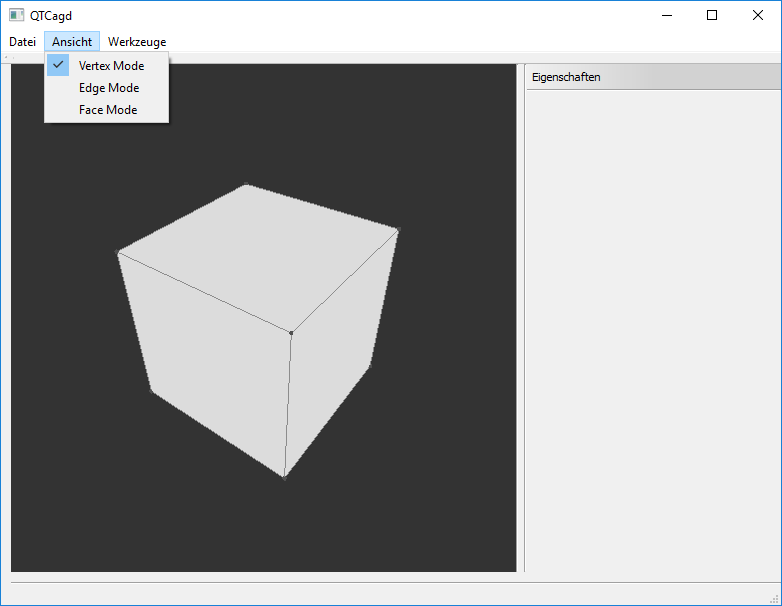
\includegraphics[width=0.6\linewidth]{content/pictures/2-Ansichtsmodi}
	\label{fig:Ansichtsmodi}
	\caption{}
\end{figure}

\subsection{Objekte selektieren}
Mit der Linken Maustaste können Grafikobjekte wie Punkte oder Kanten selektiert werden.\\
Mit Strg + Linke Maustaste kann eine Gruppe von Objekten selektiert werden.\\
Die Selektierten Objekte sind orange gefärbt.\\
Mit der Rechten Maustaste kann das ganze Mesh gedreht werden. (siehe ~\ref{fig:ObjekteSelektieren})\\

\begin{figure}[ht!]
	\centering
	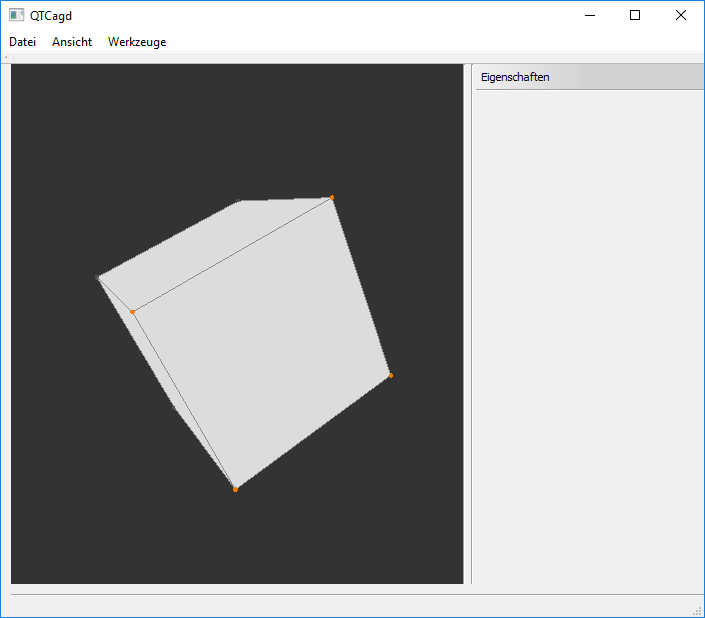
\includegraphics[width=0.6\linewidth]{content/pictures/3-ObjekteSelektieren}
	\label{fig:ObjekteSelektieren}
	\caption{}
\end{figure}

\subsection{Punkte verschieben}
Selektierte Punkte können mit gedrückter (linker) Maustaste verschoben werden.\\
Ein selektierter Punkt kann auch mit den Slidern im $"$Eigenschaften$"$ Menü verschoben werden.  (siehe ~\ref{fig:PunkteVerschieben})

\begin{figure}[ht!]
	\centering
	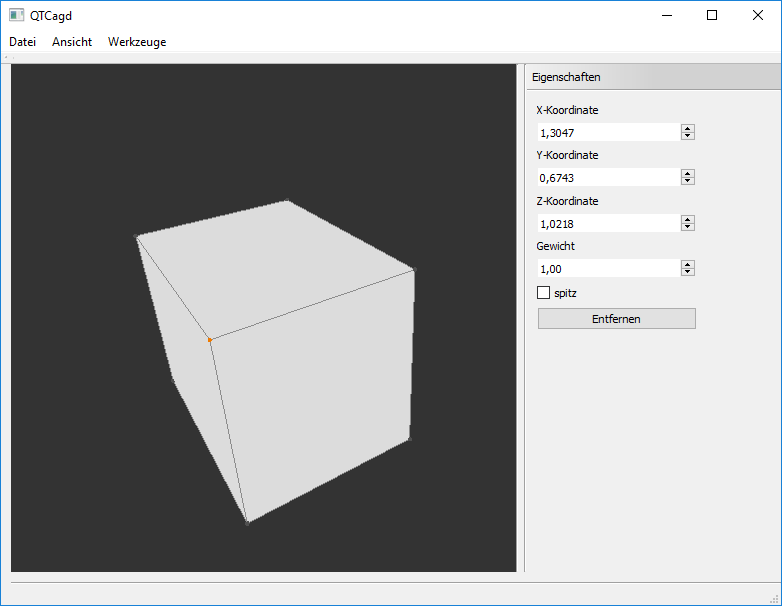
\includegraphics[width=0.6\linewidth]{content/pictures/4-PunkteVerschieben}
	\label{fig:PunkteVerschieben}
	\caption{}
\end{figure}

\subsection{Punkte löschen}
Selektierte Punkte können mit Entf gelöscht werden.
Ein selektierter Punkt kann auch mit den Button $"$Entfernen$"$ im $"$Eigenschaften$"$ Menü gelöscht werden.  (siehe ~\ref{fig:PunkteLoeschen})

\begin{figure}[ht!]
	\centering
	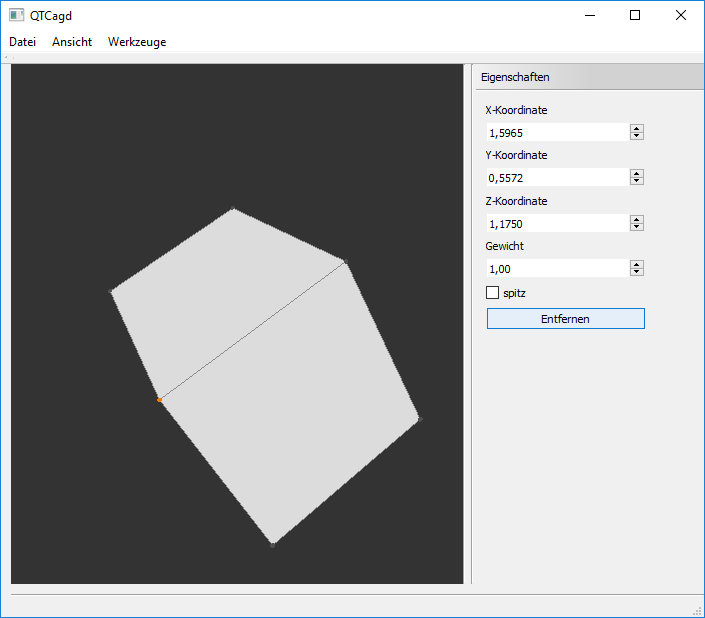
\includegraphics[width=0.6\linewidth]{content/pictures/5-PunkteLoeschen}
	\label{fig:PunkteLoeschen}
	\caption{}
\end{figure}

\subsection{Punkte gewichten}
Ein selektierter Punkt kann mit den Slider $"$Gewicht$"$ im $"$Eigenschaften$"$ Menü gewichtet werden.  (siehe ~\ref{fig:PunkteGewichten})

\begin{figure}[ht!]
	\centering
	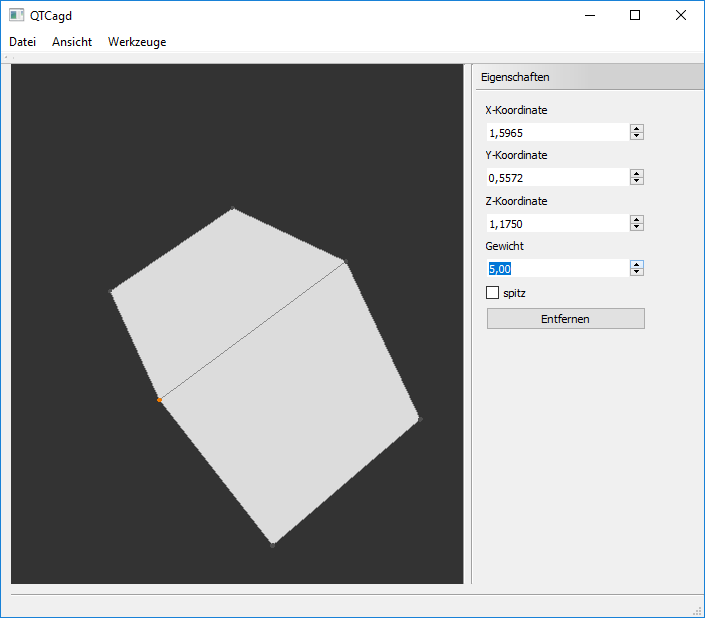
\includegraphics[width=0.6\linewidth]{content/pictures/6-PunkteGewichten}
	\label{fig:PunkteGewichten}
	\caption{}
\end{figure}

\subsection{Punkte und Kanten scharf setzen}
Ein selektierter Punkt oder selektierte Kante kann mit der Checkbox $"$spitz$"$ bzw. $"$scharf$"$ im $"$Eigenschaften$"$ Menü scharf gesetzt werden. (siehe ~\ref{fig:Punkte-KantenScharfSetzen})

\begin{figure}[ht!]
	\centering
	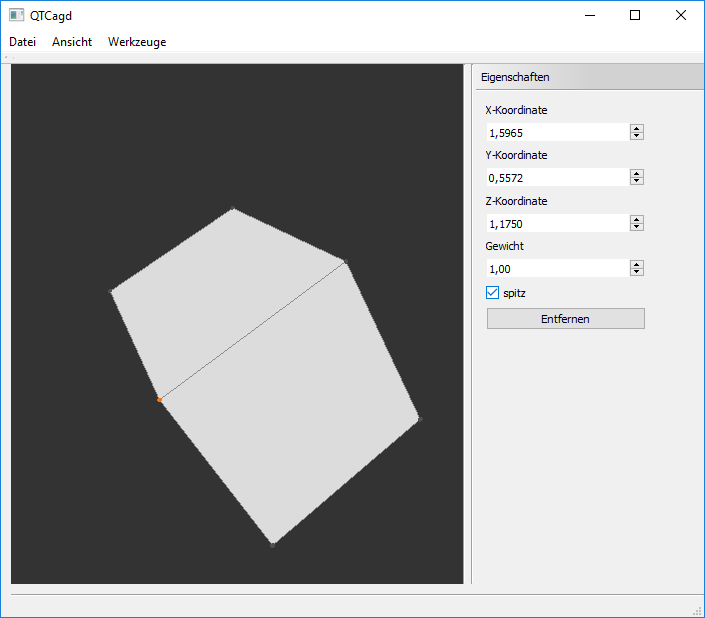
\includegraphics[width=0.6\linewidth]{content/pictures/7-Punkte-KantenScharfSetzen}
	\label{fig:Punkte-KantenScharfSetzen}
	\caption{}
\end{figure}

\subsection{Mesh mit Catmull-Clark unterteilen}
Unter $"$Werkzeuge->Catmull-Clark$"$ wird das $"$Catmull-Clark Subdivision$"$ Menü geöffnet.\\
Der Button $"$Anwenden$"$ unterteilt das Mesh. (siehe ~\ref{fig:MeshCatmullClark})

\begin{figure}[ht!]
	\centering
	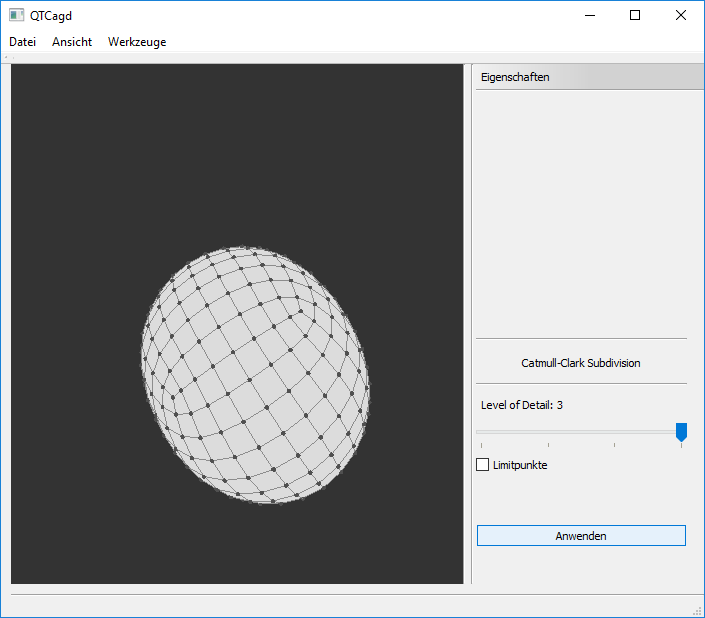
\includegraphics[width=0.6\linewidth]{content/pictures/8-MeshCatmullClark}
	\label{fig:MeshCatmullClark}
	\caption{}
\end{figure}

\subsection{Konsistenzprüfung und Statistik}
Mit der Taste $"$T$"$ kann ein Mesh auf Fehler untersucht werden und die Statistik angezeigt werden.\\
Außerdem wird nach jeder Iteration Catmull-Clark automatisch auf Fehler untersucht. (siehe ~\ref{fig:TestStatistik})

\begin{figure}[ht!]
	\centering
	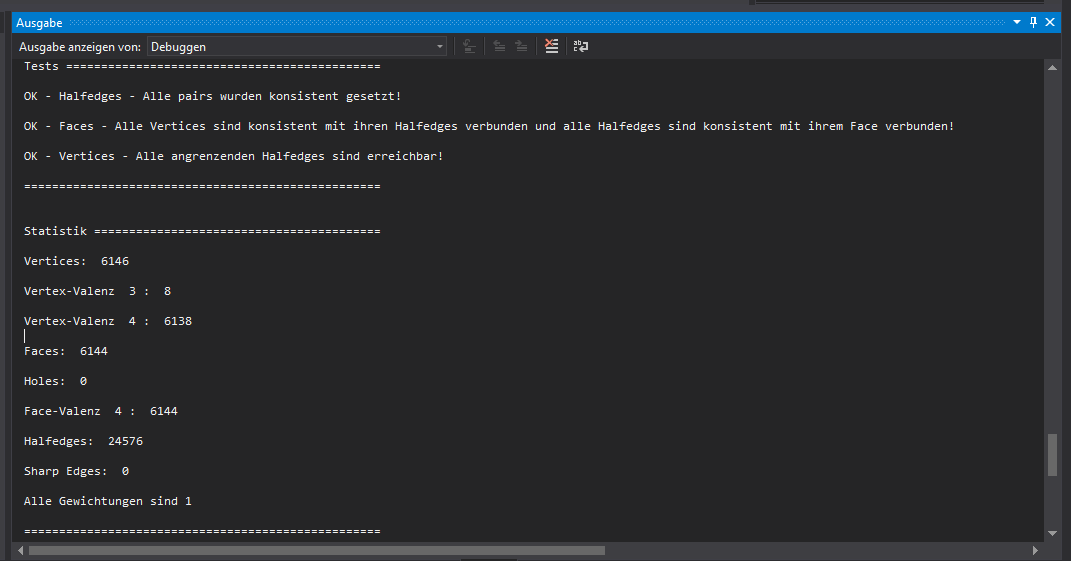
\includegraphics[width=0.6\linewidth]{content/pictures/9-TestStatistik}
	\label{fig:TestStatistik}
	\caption{}
\end{figure}
